% Configure documentclass
\documentclass[a4paper,12pt,twoside]{article}

% Add common preamble to the document
%% This file is shared between thesis and proposal

\usepackage[scaled]{helvet}
\usepackage{url}
\usepackage{cite}
\usepackage{listings}
\usepackage[pdftex]{graphicx}
\usepackage[hang,small,bf]{caption}
\usepackage{styles/tum}
\usepackage{setspace}
\usepackage[german,english]{babel}
\usepackage{float}
\usepackage{floatflt}
\usepackage{fancyhdr}
\usepackage{color}
\usepackage{booktabs}
\usepackage[pdftex,bookmarks=true,plainpages=false,pdfpagelabels=true]{hyperref}	%TODO make yourself familiar with \label, \ref and \hyperref for referencing figures, tables, chapters, etc.
\usepackage{mdwlist}
\usepackage{enumerate}
\usepackage{array}
\usepackage{longtable}
\usepackage[utf8]{inputenc}
\usepackage[capitalize, noabbrev]{cleveref}
\usepackage{wasysym}
\usepackage{todonotes}

% Path for graphics
\graphicspath{{figures/}}

% Include the Thesis metadata like title, author, etc. 
\input{metadata}

%%%%%%%%%%%%%%%%%%%%%%%%%%%%%%%%%%%%%%%%%%%%%%%%%%%%%%%%%%%%%%%%%%%%%%%%%%%%%%%%%%%%%%%%%%%%%%%%%
% Custom Commands for this template
%%%%%%%%%%%%%%%%%%%%%%%%%%%%%%%%%%%%%%%%%%%%%%%%%%%%%%%%%%%%%%%%%%%%%%%%%%%%%%%%%%%%%%%%%%%%%%%%%

% Annotate feedback you received 
\newcommand{\feedback}[1]{\todo[inline,color=green,caption={}]{#1}}

% State what is missing in this spot
\newcommand{\missing}[1]{\todo[inline,color=yellow,caption={}]{#1}}

% Inline to do note: 
\newcommand{\TODO}[1]{\todo[inline,caption={}]{#1}}





\def\proposal{Proposal for}

%%%%%%%%%%%%%%%%%%%%%%%%%%%%%%%%%%%%%%%%%%%%%%%%%%%%%%%%%%%
% Theses specific packages go here
%%%%%%%%%%%%%%%%%%%%%%%%%%%%%%%%%%%%%%%%%%%%%%%%%%%%%%%%%%%
\usepackage[nolist]{acronym}
\usepackage{titlesec}
\usepackage{graphicx}
\usepackage{caption}
\usepackage{hyperref} % to handle URLs and create hyperlinks
\usepackage{enumitem} % for customizing lists
\newcommand{\sectionbreak}{\clearpage}

%%%%%%%%%%%%%%%%%%%%%%%%%%%%%%%%%%%%%%%%%%%%%%%%%%%%%%%%%%%
% Begin of document
%%%%%%%%%%%%%%%%%%%%%%%%%%%%%%%%%%%%%%%%%%%%%%%%%%%%%%%%%%%
\begin{document}
\setlength{\evensidemargin}{22pt}
\setlength{\oddsidemargin}{22pt}


\hypersetup{pdfborder={0 0 0}, pdfauthor={\author}, pdftitle={\title}}

\lstset{showspaces=false, numbers=left, frame=single, basicstyle=\small}

%------- Title setup -------
\thispagestyle{empty}
{
\sffamily

\vspace{1cm}
\begin{center}
\oTUM{4cm}

\vspace{5mm}     
{\LARGE \bf \sffamily Technical University of Munich}

\vspace{5mm}
{\Large School of Computation, Information and Technology \\ -- Informatics -- }	
\vspace{1mm}
\end{center}

\vspace{15mm}

\begin{center}
        {\large {\proposal} {Bachelor}'s Thesis in \program}
\vspace{8mm}

\begin{spacing}{1.3}
{\LARGE \bf \sffamily Enhancing Contextual Awareness of IRIS: Incorporating Lecture Content into a GPT-based Educational Chatbot on the Artemis Learning Platform}\\
\vspace{8mm}

{\LARGE Erweiterung des Kontextverständnisses von IRIS: Integration von Lehrinhalten in einen GPT-gestützten pädagogischen Chatbot innerhalb der Artemis-Lernumgebung}\\
\vspace{8mm}
\end{spacing}

\begin{tabular}{ll}
\large Author:           & \large Yassine Souissi     \\[2mm]
\large Supervisor:       & \large Stephan Krusche \\[2mm]				
\large Advisor:	         & \large Patrick Bassner    \\[2mm]
\ifx\proposal\empty\else
\large Start Date:       & \large 15.11.2023  \\[2mm]
\fi
\large Submission Date:  & \large 15.03.2023
\end{tabular}

\end{center}
}

\selectlanguage{english}
\pagenumbering{arabic}

\fancyhead{}
\pagestyle{fancy}
\fancyhead[LE]{\slshape \leftmark}
\fancyhead[RO]{\slshape \rightmark}
\headheight=15pt

%------- Start of Proposal -------
\section{Introduction}
            
            In the dynamic realm of higher education, platforms likeCoursera\footnote{\url{https://www.coursera.org/}}, Udacity\footnote{\url{https://www.udacity.com/}}, and Khan Academy\footnote{\url{https://www.khanacademy.org/}} have already set the stage for a global educational network, connecting students and educators like never before. However, in conventional university contexts, especially in large-scale courses such as Computer Science, the need for personalized academic support remains unmet.
            
            Addressing this gap, the Technical University of Munich is at the forefront of educational innovation with the development of Artemis\footnote{\url{https://artemis.ase.in.tum.de/}} and IRIS. Artemis, designed to be flexible and scalable, accommodates extensive student cohorts with features such as live streaming, interactive quizzes, and automated exercise evaluations.\cite{3} These innovations aim to assist educators in managing the increased demands of course delivery and in sustaining the integrity of educational feedback mechanisms.\cite{4}
            
            Adding to this transformative landscape is the introduction of IRIS, an intelligent virtual tutor. Embedded within Artemis, IRIS represents a leap towards AI-driven interactive learning. Leveraging Generative AI and Large Language Models (LLMs), IRIS is specifically tailored to aid students in solving programming tasks. This virtual tutor is not just a repository of information but an interactive tool that provides one-on-one assistance, fostering deep understanding and autonomy in solving programming exercises. 
            
            With Artemis and IRIS, the Technical University of Munich is not just responding to the challenges of modern education but redefining the very essence of learning in the digital age. These platforms symbolize a future where education is more adaptive, responsive, and effective, tailored to students' diverse and dynamic needs worldwide. 
     
    
                
\section{Problem}

Within the Artemis initiative, the Computer Science education sector is confronting significant challenges that undermine the student learning experience. Despite the support from teaching assistants, a dedicated chair, and tutors, there is a notable deficiency in personalized academic support. This shortfall is largely attributed to the soaring enrollments, often surpassing 1000 undergraduates and 500 postgraduates, which stretch the educators' capacity to provide prompt and individualized responses an essential element for effective learning.\cite{1}

Exacerbating this situation is the widespread use of standardized lecture materials. These materials, designed for mass dissemination, fail to cater to the diverse educational needs and backgrounds of a large student body. Consequently, this one-size-fits-all approach leaves many students lacking in necessary, personalized academic assistance.

A further complication is the difficulty in providing immediate responses to student inquiries during lectures. This challenge stems not only from the educators' limited capacity to address so many questions in real time but also from students' reluctance to ask questions, possibly due to fear of judgment or the sheer volume of queries. Such impediments in timely communication hinder students' comprehension of vital Computer Science concepts, adversely affecting their academic development.

In the midst of these challenges, IRIS currently provides feedback on programming exercises and aids in the understanding of related concepts. However, IRIS's functionality is constrained by its lack of awareness of the lecture content, limiting its ability to offer comprehensive support tailored to the curriculum. As a result, while IRIS serves as an invaluable tool for certain aspects of the learning process, its potential remains partially untapped in the broader educational context.

        
\section{Motivation}
       The imperative to enhance Computer Science education is highlighted by the inadequacies of traditional teaching methods in large-scale academic settings.

        Traditional interactive learning methods falter under the weight of large student numbers, where personalized engagement is challenging. IRIS is designed to overcome these barriers, offering scalable and adaptive interactions that cater to individual student needs, a feat unattainable in extensive lecture formats.

        The absence of adequate guidance is a recognized impediment in the learning process.\cite{3}\cite{5} IRIS seeks to mitigate this by providing immediate, tailored assistance, enabling students to navigate the intricacies of Computer Science education effectively. This support is crucial for preventing the development of misconceptions and ensuring a robust conceptual understanding.

        Embracing a student-centered learning approach, IRIS is envisioned to foster an educational environment that adapts to the diverse requirements of learners. This strategy enhances inclusivity and encourages students to actively participate in their educational journey.

        Additionally, the insights gleaned from student interactions with IRIS offer educators actionable data to refine and optimize lecture content. This feedback loop is essential for the ongoing enhancement of course material and teaching strategies.

        The enhancement of IRIS represents a significant advancement in addressing the prevalent challenges within Computer Science education. It promises to elevate the quality of learning experiences and prepare students to thrive in a dynamic landscape.
        
\section{Objective}
The focus of this thesis is to enhance the contextual awareness of IRIS by incorporating lecture content into the GPT-based educational chatbot on the Artemis Learning Platform. This development aims to streamline IRIS's ability to address student inquiries related to lecture content more effectively. The focus here is on leveraging the existing integration of GPT-3.5 in IRIS and enriching it with a structured, easily accessible vector database of lecture materials.\cite{6}

By embedding these materials into a vector database, IRIS will be equipped to perform more accurate and relevant searches in response to specific student queries. This process involves the creation of lecture content embeddings, ensuring that IRIS can efficiently access and utilize this information during student interactions. 

The project will adhere to best practices in software engineering. The deliverables of this thesis will be a fully functional integration of the vector database with IRIS, and documentation detailing the design and implementation process. The aim is to demonstrate how this enhancement can provide more precise and contextually relevant support to students, thereby enriching their learning experience and potentially reducing the workload on human tutors. 

\subsection{Proposed High-Level Workflow}
Proposed High-Level Workflow

Upon receiving a query, the Large Language Model (LLM) promptly processes the input, transforming the natural language question into a query embedding. This embedding will be the basis for a semantic search within the knowledge base, which is to be constructed utilizing a vector database capable of housing the pre-encoded lectures.
The semantic search executed by Artemis delves into the vector database, retrieving a ranked list of results pertinent to the user's query. These results are critically analyzed by the LLM, which then crafts a coherent and contextually relevant response.\cite{6} This interaction is envisioned to be depicted in an activity diagram, as outlined in Figure 2.

In the selection of the vector database, OpenAI's recommendations will be taken under advisement, with the final choice being contingent upon a multifaceted evaluation. Criteria such as extensibility, performance, integrability, and sustainability will be paramount in this decision-making process. The goal is to ensure that the database not only meets the current functional requirements but is also robust enough to support future expansions and integrations.

During the processing of student questions, a specialized prompt for the LLM will be developed to effectively extract and interpret relevant lecture content. This prompt will be tailored to understand the context of each inquiry, ensuring that the responses provided are both accurate and directly relevant to the specific content of the lectures.

\begin{figure}[ht]
\centering
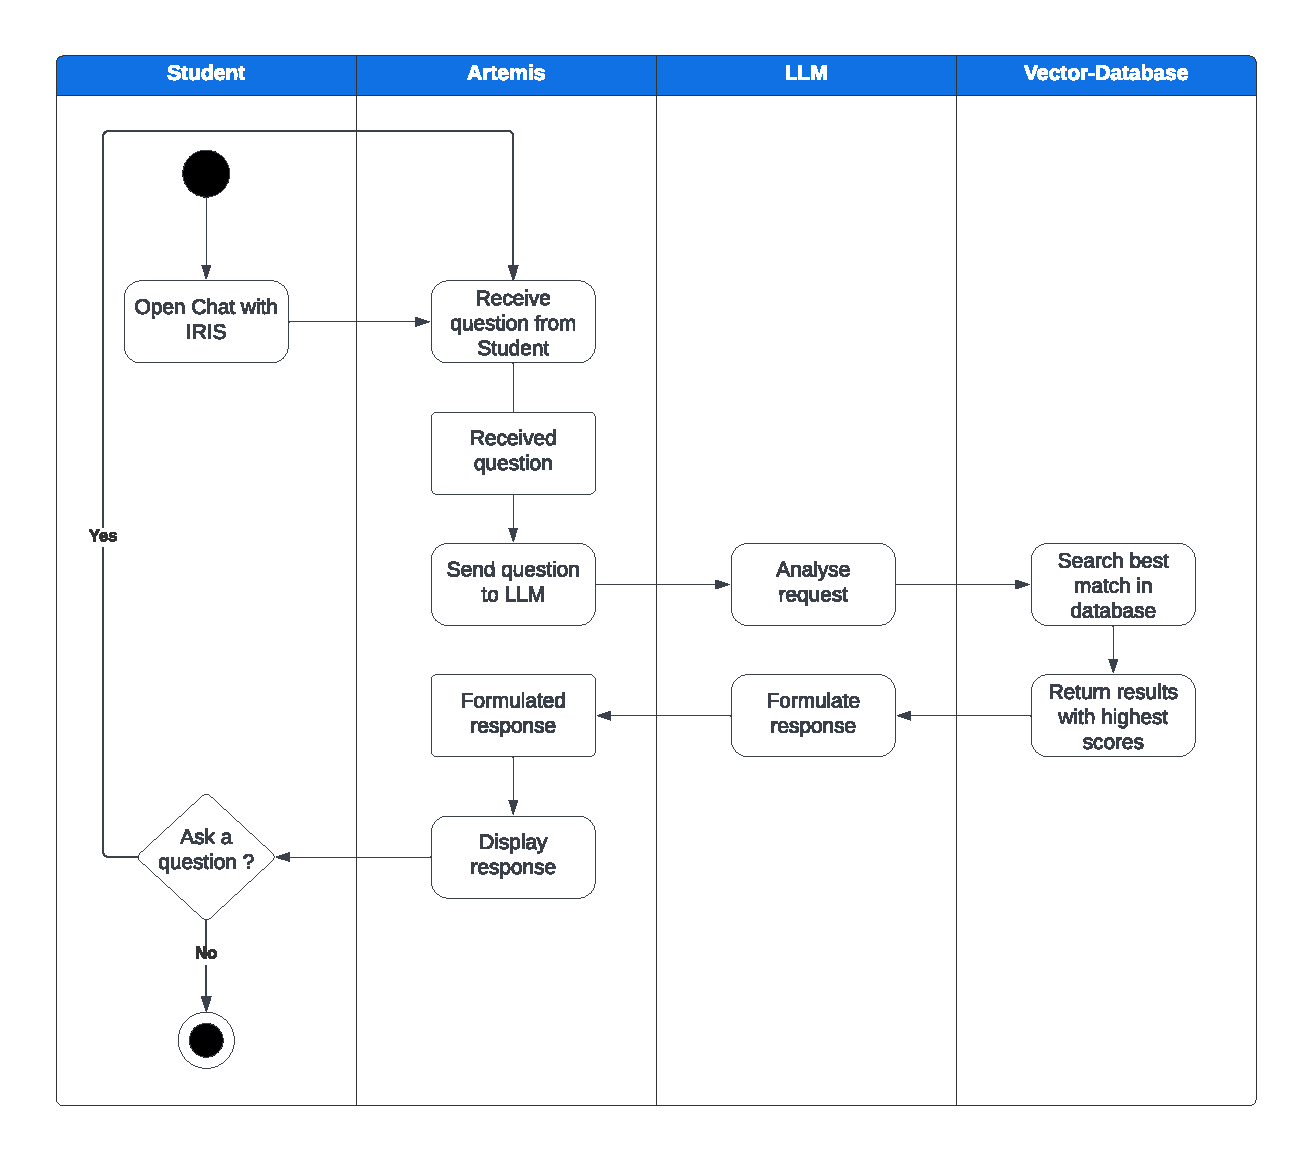
\includegraphics[width=1.1\textwidth]{Proposal Activity Diagram.pdf}
\captionsetup{font=small, labelfont=bf, justification=centering, format=plain}
\caption[Short version for List of Figures]{A detailed description of the diagram that serves as a legend.}
\label{fig:diagram}
\end{figure}




\section{Schedule}
\begin{itemize}
    \item \textbf{15.11 Thesis Kickoff}
    \item \textbf{Until 01.12: Initial Requirement Synthesis and Concept Validation}
    \begin{itemize}
        \item Perform an exhaustive evaluation of the project's prerequisites, covering both the technical framework and functional specifications.
        \item Assess a range of established methodologies and Language Model paradigms for their suitability in achieving the project’s goals.
        \item begin implementing A Minimal Viable Product for testing.
    \end{itemize}
    \item \textbf{Until 15.12: Core Prototype Construction )}
    \begin{itemize}
        \item Develop an elementary prototype in Python to showcase the essential capabilities of the Language Model with integrated long-term memory features, fulfilling the defined criteria.
    \end{itemize}
    \item \textbf{Until 01.01: Enhanced Prototype Development}
    \begin{itemize}
        \item Engineer an additional prototype with minimal viable functionality, utilizing Python to exhibit foundational Language Model operations coupled with extended memory functionalities, conforming to the established requirements.
    \end{itemize}
    \item \textbf{Until 15.01: Comparative Analysis and Integration Selection}
    \begin{itemize}
        \item Execute a comprehensive evaluation of the employed technologies and elect one for integration into the Artemis framework.
        \item Begin the integration into Artemis.
    \end{itemize}
    \item \textbf{Until 01.02: Finish the integration into Artemis and begin testing}
    \begin{itemize}
        \item Undertake extensive validation by integrating the prototype into the Artemis ecosystem to confirm seamless incorporation and functionality.
        \item begin testing the product with the Artemis team.
    \end{itemize}
    \item \textbf{Until 15.02: Integration within Artemis }
    \begin{itemize}
        \item incorporate the feedback from the Artemis team
        \item begin testing the product with together with the students.
    \end{itemize}
    \item \textbf{Until 01.03: Finalization and Pre-Deployment Optimization }
    \begin{itemize}
        \item Allocate this period for rigorous debugging, rectification of any aberrant behavior, and refinement to a polished Minimum Viable Product (MVP).
        \item Prime the project for a seamless transition into the operational phase during the forthcoming Summer Semester 24/25, ensuring its deployment readiness.
        \item Compile exhaustive user manuals and documentation to ensure a smooth transition into active use.
    \end{itemize}
\end{itemize}

\clearpage
\begin{acronym}
\acro{GUI}{Graphical User Interface}
\end{acronym}

\clearpage
\bibliography{thesis}

\bibliographystyle{alpha}

\end{document}
